\documentclass[a4paper,12pt]{Article}
\usepackage{witsa4}
\usepackage{times}
\usepackage{graphicx}
\usepackage{graphics}
\usepackage{amsmath, amsthm, amsfonts, amssymb, graphicx, color, epsfig,float, url}
\usepackage{hyperref}


\usepackage{url}
\usepackage{natbib} \input{natbib-add}
\bibliographystyle{named-wits}
\bibpunct{[}{]}{;}{n}{,}{,}  % to get correct punctuation for bibliography

\title{Group Project Report\\ Software Techniques and Technologies \\ELEN7046 \\Unit Test Visualization}
\author {Group 4 \\ Boreli Kuleile \\Demi Ojurongbe\\Keagan Phillips\\Sello Ralethe\\Xoliswa Ngxanga\\\\\\\\\\\\\\\\{Source \& Documentation: https://github.com/KeaganPhillips/Wit-Group-4-project }


\begin{document}
\pagenumbering{roman}
\setcounter{page}{0}
\maketitle
\newpage
\section*{Declaration}
We declare that this is our work, any and all third party components have been referenced considering licensing. It is being submitted towards the completion of the ELEN 7046 course, to the School of Electronic and Information Engineering at the University of the Witwatersrand, Johannesburg. It has not been submitted before for any degree or examination to any other University.
\\\\The Group has also agreed to the following discretionary points allocation:
\begin{itemize}
\item Boreli - 5 points
\item Demi - 5 points
\item Keagan - 5 points
\item Sello - 5 points
\item Xoli - 5 points
\end{itemize}
\\\\Signatures
\\\\\\\\\\\\Date
\newpage

\begin{abstract}
The design and implementation of a software visualisation tool for unit testing is presented. The visualisation tool is to be used to graphically display, enhance and simplify unit tests. The development of both the unit tests and its visualisation are discussed. The tool was implemented using TDD and uses C\# Reflection to obtain the necessary information which was then sent to the visualiser to display. The implementation suggests that the tool can play an important role in software visualization education.
\end{abstract}
\newpage

\tableofcontents
\listoffigures
\pagenumbering{arabic}

\newpage
\section{Introduction}
This paper presents a report of an application that links software visualisation and software education. In the literature, it is stipulated that software visualization encompasses the development and evaluation of methods for graphically representing different aspects of software, including its structure, its execution, and its evolution.\\
\linebreak  
The aspect of software that we present in this report is Unit Testing\cite{unitTests}. The primary goal of unit testing is to take the smallest piece of testable software in the application, isolate it from the remainder of the code, and determine whether it behaves exactly as expected. Each unit is tested separately before integrating them into modules to test the interfaces between modules.
This testing mode is a component of Extreme Programming (XP)\cite{xp}, a pragmatic method of software development that takes a precise approach to building a product by means of continual testing and revision.\\
\linebreak  
Unit testing involves only those characteristics that are vital to the performance of the unit under test. This encourages developers to modify the source code without immediate concerns about how such changes might affect the functioning of other units or the program as a whole. Once all of the units in a program have been found to be working in the most efficient and error-free manner possible, larger components of the program can be evaluated by means of integration testing.\\
\linebreak  
In this report, we primarily demonstrate an application that visualises all the unit tests in a given program. The application discussed in this report visualises not only the unit tests, but also the class diagrams together with their public methods and properties.\\
\linebreak  
The remainder of this report is as follows. Section 2 discusses the licenses used in the development of the application. We provide the problem description in section 3, and discuss the approach we took to solve the problem in section 4. Installation process for the application is discussed in section 5. We provide a discussion on how the approach to the solution was implemented in section 6. In section 7, we discuss an analysis of our solution, and provide future works in section 8. We end the report with a conclusion
\section{License Agreement}
\subsection{Overview}
An analysis of software licenses was done considering the combination of both original work and third party components. The new BSD license also known as the 3-Clause BSD\cite{bds} license was chosen. The software and source code are made available under this license. Use, modification and redistribution is not restricted. 
\subsection{Components used and their license agreements}
The following lists the components used within the system together with their respective license agreements.
\begin{itemize}
\item \textbf{Coffee Script}: MIT license\cite{mit}
\item \textbf{Java script:} GNU GPL\cite{gnugpl}
\item \textbf{JQuery:} GNU GPL\cite{gnugpl}
\item \textbf{Kinetic.js:} GNU GPL\cite{gnugpl}
\item \textbf{PDF reporting tool:} CPOL\cite{cpol}
\item \textbf{ITextSharp:} GNU GPL\cite{gnugpl}
\end{itemize}

For the complete reference, please refer to the document 'ELEN7046 - Group4 - Licence Agreement.pdf'\cite{licenceDoc}


\section{Problem Description}
\subsection{Overview}
As good software practitioners, we always aspire to adopt the current best practices in our industry. In recent years the so called 'Agile' methodologies has become very popular with TDD\cite{tdd} (Test Driven Development) begin a very widely adopted agile practice. Today it is almost expected of developers to not only write program code, but also create automated unit tests and apply other TDD practices.
\subsection{Problems with respect to Unit Tests}
Writing automated unit tests comes with its own unique problems. Our project attempts to address some of these shortcomings by proposing a framework against which developers can write their automated tests. The end result should give developers a broad and high level view of all unit tests, making it easier for them to get a holistic view of all the unit tests in the system under test.
\subsubsection{Large Complex projects}
Tests can become difficult to read and understand especially as the suite of tests rapidly grows in number and complexity with each build deployed. It is very easy for a developer to get lost in the detail by reading the actual automated test code. This is because the developer can only view one automated unit test at a time, making it difficult to see the whole picture. 
\subsubsection{Comments in tests}
Many developers don't write adequate comments in their tests leaving other team members in the dark with regard to what their initial intent was.\\
\linebreak
It's never good to have a test or group of tests that isn't well understood (even though the test(s) may pass). Tests are only useful when the context of the tests is clear and well understood.  
\subsubsection{The Learning Curve}
The above described scenarios make it difficult for the development team to evolve a system over time. The result being that the learning curve is often very steep for new developers joining the development team as well as for junior developers on the team.
\subsection{Proposed Solution}
What is needed is a framework that provides a convention that developers can follow where tests are written in a uniformed way. The system must provide a mechanism to visually display all tests without the developer having to zoom into the code to look at tests one at a time.\\
\linebreak
This, we believe should add tremendous value with respect to the learning of an existing and evolving code base.

\section{Approach}
Given the above stated requirement, the team proposed the following solution. A web application will be developed that provides a visual representation of the unit tests of the system under development

\subsection{High level design overview}
Figure \ref{fig1} depicts a high level overview of the proposed solution. This section will briefly discuss the key components of the system from right to left.

\begin{center}
	\begin{figure}
		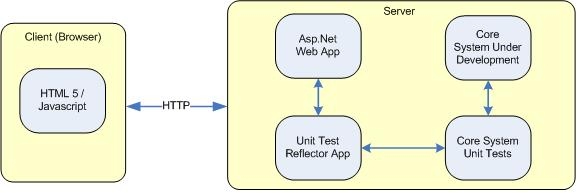
\includegraphics{system_overview.JPG}
			\caption{}
			\label{fig1}    
	\end{figure}	
\end{center}

\subsubsection{Core System Under Development}
This component represents the actual core application. This is the system that will actually run in the production environment and the application against which the unit tests will run. This system is completely oblivious of the other components depicted. Obviously developers must use an "interface driven" approach upon developing this component to facilitate modularity and enable for easy unit testing. The actual functional requirements for this application is beyond the scope of the project.\\
\linebreak
Please see section 3.1 of Keagan Phillips's individual report\cite{reportKeagan} for more a more in depth discussion regarding this component. 

\subsubsection{Core System Unit Tests}
This component represents the actual unit test project and contains automated unit tests. These tests target the "Core System Under Development" component.\\
\linebreak  
Tests must be written following a predefined convention\cite{UTconvention}. The development team used the TDD\cite{tdd} (Test Driven Development) technique and "Given / When / Then"\cite{gwt} convention for specifying tests scenarios.\\
\linebreak  
Please refer to section 3.2 of Keagan Phillips's individual report\cite{reportKeagan} for more detail on this component.\\
\linebreak  
Please see the "Unit Test coding convention" document for an in depth discussion on how to wire automated tests using the provided framework.\cite{UTconvention}

\subsubsection{Unit Test Reflector}
This component's responsibility is to extract the unit test metadata embedded in the "Core System Unit Tests" component and transform that data into a C\# data structure. The team made use of the Microsoft Dot Net Framework's Reflection\cite{reflection} feature to achieve this goal. This data can then be collated and presented to the user in almost any format including document format (i.e. HTML page or PDF) or in our case visually and in pdf format as shown later on.\\
\linebreak  
Please refer to section 3.3 of Keagan Phillips's individual report\cite{reportKeagan} for more detail on this component.\\ 

\subsubsection{Asp.Net Web Application}
This component acts as a shell to host our solution in a web based environment. It calls the component 'Unit Test Reflector Application' upon receiving a web request. It then retrieves a data structure with the relevant test metadata. The data is then converted from a dot Net C\# object, to a JSON\cite{json} data structure to be transmitted back to the browser as an HTTP response.\\
\linebreak  
See Borelli’s report for more information.\cite{reportBoreli}

\subsubsection{HTML5 / Javascript Component}
This is the front end component responsible for the actual user interface, the layout and presentation logic. It sends an HTTP request to the 'Asp.Net Web App' component and expect a JSON\cite{json} structure back. The data retrieved from the web server is then bound to the user interface giving the user a visual representation of the unit tests.\\
\linebreak
Please refer to Sello's\cite{reportSello} and Demi's\cite{reportDemi} individual reports for more regarding this component.

\subsection{Screen Layout}
The main screen is segregated into three main sections. We will now briefly describe these section. The Figure \ref{fig2} is a 'mock-up' representation of the proposed screen. 


\begin{center}
	\begin{figure}
		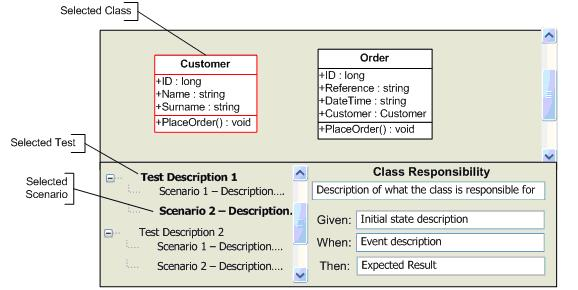
\includegraphics{screenmock.JPG}
			\caption{}
			\label{fig2}    
	\end{figure}	
\end{center}


\subsubsection{Class diagram canvas}
The \textbf{Class diagram canvas} represents the top half section in Figure \ref{fig2}. This section will display interactive movable lightweight class diagrams. One class diagram will get created for each class being tested. The class diagrams must be selected. The selected class must be highlighted to distinguish it from other classes.\\
\linebreak 
See Sello’s\cite{reportSello} report for more information on the implementation of this screen.

\subsubsection{Treeview panel}
The \textbf{Treeview Panel} is represented on the bottom left section in Figure \ref{fig2}. This section will be empty initially and will only populate when the user selects a class diagram. The main purpose of this section is to present to the user a tree view control listing all the tests for the selected class and each test's related test scenarios. This panel will refresh with new content when the user selects another class from the class diagram canvas.\\
\linebreak
See Demi’s\cite{reportDemi} report for more information related to this screen.

\subsubsection{Details view panel}
The \textbf{Details view panel} is represented on the bottom right section of Figure \ref{fig2}. The panel will initially be blank and will only populate when the user select a scenario from the tree view control. It will display data related to the scenario selected (i.e. the Given / When / Then details) amongst other details including the class name; class description; and other test related details\\
\linebreak
See Demi’s\cite{reportDemi} report for more information related to this screen.


\section{Installation Process}
The Installation guide can be found on the group website under section Installation. The file name is ELEN 7046 - Installation Guide.pdf 
\section{Methodology}
\subsection{Project Methodology }
The nature of the project required our approach to be lean and agile, because of the fixed time and the availability of of the team members. As team 4 we decided on the Kan-Ban development methodology  because it is one of the most lightweight development methodologies  and it puts an emphasis on just-in-time  delivery .
\\\\The methodology allows the users to tailor it to their own requirements  because it contains no specific roles or processes, and it encourages incremental development. The methodology helped us to visualize the work flow, the entire team could always see what is currently being done, what was complete and what was still outstanding. This helped us to keep the big picture in mind as we collaborated .It also assisted us in eliminating waste , amplifying learning and empowering the team members which are some of the key principles of lean development.
We used the free Kanbanery tool to help us track our Kanban board. We chose this tool because it is easy to use and it has a better  graphical user interface compared to other freeware alternatives. The freeware version had its own limitations therefore we supplemented it with open proj , a freeware project management tool which enabled us to perform tracking  in more detail. For more information on the project methodology and management refer to Xoliswa’s individual report.
\subsection{Requirements Methodology}
The main purpose of the system requirements document is to formally document the requirements of the system being developed [6]. It aids communication between the developers and the users of the system , detailing  what is expected of the system. The document is important to the group because it serves as a clear starting point that enable communication amongst team members .
\\\\The scope of the project is to provide a visual representation of classes, test cases, scenarios and conditions. The benefit that will be achieved by the user of the system after successful completion is that the user will spend less time scanning through the code to find tests, and the user will have a more global understanding of the project under test.
\\\\The document also details the assumptions we made , the inclusions, exclusion , user interfaces, report requirements , and use cases for the system. For more information on the details of the document  please refer to the system requirement document and Xoli’s report.
\subsection{Design Methodology}
From the above section, the problem description, a high level overview of the proposed solution is given. The coding tasks were broken down into these different components but were not strictly isolated into silos, as the peer programming approach was employed in certain areas to increase learning capabilities. These areas are the front-end application, the back-end application and the core system 
\subsection{Coding Methodology}
\subsubsection{Technology Stack} 
\begin{itemize}
\item CoffeeScript
\item Javascript 
\item Jstrees and tree view controller
\item JSON
\item HTML5
\item PDF reporting tool
\item GIT
\end{itemize}
CoffeeScript and javascript are both scripting languages that are used to add more functionality to HTML pages and also improve interactivity. CoffeeScript is a minimal language that compiles to JavaScript. It aims to expose the good parts of JavaScript in a simple way. For more information on CoffeeScript, see Sello’s report.
\\Jqtrees are a type of javascript tree, and the Jqtrees made the best fit for the application and were easily integrated into the application. The Jqtree is a tree widget, which creates a tree from JSON data [5]. The tree is written in javascript  in a scripting file in the HTML file. The tree view controller is then used to manipulate the created tree, it also enables features on the tree, see Demi's report.
\\HTML5  is the fifth major revision of HTML.Unlike older versions of HTML, this new one is designed to do more things. For instance, animations can be displayed directly in the browser without a plugin. A more comprehensive discussion of HTML5 and how it was used in the project can be found in Sello’s report.
\\GIT is the repository the development team used to work from different geographical locations. It is a distributed repository system
\subsection{Testing Methodology}
Our testing methodology was influenced  by  the template prescribed for test driven development.  The developers executed unit testing for the various components of the system , integration testing was carried out every time changes were  incorporated into the system.
\\We also did regression testing to ensure that the newly incorporated components did not break the existing components that had already passed testing. 
\\\\A final system test was carried out to verify if the system met the requirements as stated in the systems requirements document. The results from the test can be found in the test report document. For information on our testing decisions and analysis consult Xoli’s report.

\section{Future Work}
This section identifies some of the areas of the application which were not covered or attempted and incomplete. These will be added by the team or any other developer who wants to improve the application. Another developer is permitted to make modifications and still distribute, this is granted by the licence on the application. The new / 3-clause BSD licence.
\begin{itemize}
\item The application can be expanded to cater for applications under test which are written in other languages.This was not possible within the time frame the group was given to implement the project. Currently the application under test is written in the C\# programing language using Visual Studio. To expand this to cater for applications under test written in different language, say the Java programming language, the Unit test reflector component of the application will be re-written in Java and it will instead look for JUnit tests also known as Java unit tests. This way the application will then be able to reflect over an application under test written in the Java programming language. This is possible in other Object Oriented languages as well, and to execute this the unit test reflector component of the application will be written in the respective language and will produce the JSON data structure the same way and will be sent to the front end.
\item The next possible improvement or feature for future work will be to complete the application under test which currently exists in the application. This was not completed due to a slight overestimation on the groups planning. Currently the application under test is a banking atm application. The application has only a required set of features to efficiently perform unit tests. To complete or extend this, the ideal situation will be to have the complete banking atm application to run tests over, as there may be tests which the actual system needs which were not considered or discovered by the development team - group 4. This was also given less preference in development as it was also considered out of the scope of the project, not directly adding value to the software education or visualisation of the project.
\item The next feature here is currently being worked on by the group, till submission. This is to ensure that the application works in all browsers. The application currently works smoothly in the Google chrome browser, which the team was using during development and testing. The application does have a few bugs when run in Internet explorer and Firefox. This will be or can be done by fixing the current bugs which prevent it from running in internet explorer and Firefox.
\item The final set of features here are to improve the visualization experience and educational value. To do this, the team was to add the following features to the user interface (browser):
\begin{enumerate}
\item The team suggested adding a button to the screen to enable the user user to run the actual unit tests, given the particular scenario which they have chosen. In doing this the user then gets a result as to whether the unit test was passed or not. This button will call the unit tests in the back end which will run and the messages usually displayed to the console will be directed to a panel on the screen. Displaying this will also inform the user as to reasons why the test may have failed the test, identifying possible bugs in the application under test.
\item A trivial one, though completely overlooked, is to add a button which clears the screen. This differs from reloading the page, here the user will not have to reload the page but just clear the screen, meaning that the data sent to the front end has not been cleared or overwritten.
\item To improve the educational value, the team would add a menu to the screen, allowing the user to select from a range of theoretical information and examples including source code which the user can also use to learn more about unit tests. In doing so the user is then able to select well explained documentation on what a unit test is, why it is used and how to implement it efficiently.
\end{enumerate}
\end{itemize}
These features are some and not all of the possible improvements to the application. These were identified by the group and would have been implemented possibly with a wider time frame. Nevertheless the group feels the application does give a good account of the ideas that were conceived and developed in the process.

\section{Conclusion}
The objective of visualizing the unit tests was achieved in the project. The visual representation of the class diagrams for the unit tests as well as the display of the test case scenarios on the report were displayed as planned. Apart from the improvements that may need to be made in future as stated in future work section, all of the milestones set were achieved. The developers are able to visualize the individual unit tests together with the accompanying class diagrams with methods and properties.  They are able to check unit tests without going through the code that is hard to understand mostly by new developers. The other aspect that is not covered due to time constraint is to make the web application more appealing. JqueryUI was attempted to make good looking front page but could not work unfortunately.
\\\\Most skills required in software development projects were acquired by the team members. Technical, management and teamwork are some of the skills acquired during the project. Though the project had numerous challenges and issues, it exposed the group to an array of new and different tools, technologies and techniques. The technologies and tools used in software development were tested and put into practice.  All in all the project has been the great learning experience for all the members and everyone has benefited in their own right.
\\\\The group feels that the solution presented is a great way to illustrate software visualisation and/or education. 











\newpage

\begin{thebibliography}{99}
\addcontentsline{toc}{chapter}{\protect References}



\bibitem[1]{unitTests} Extreme Programming (2012),``Unit Tests", \textit{Rules} \url{http://www.extremeprogramming.org/rules/unittests.html}, Last accessed June 2012.

\bibitem[2]{xp} Extreme Programming (2012), ``Unit Tests", \textit{Lessons Learned}\url{http://www.extremeprogramming.org/}, Last accessed June 2012.

\bibitem[3] {bds} Open Source Initiative, Various authors (2012),``The BSD License", \textit{Open Source Initiative},\url{http://www.opensource.org/licenses/BSD-3-Clause}, Last accessed June 2012.

\bibitem[4]{licenceDoc} \textbf{ELEN 7046 group license}, (2012) ,``Group Project Licence Choice", \textit{Software Licensing}.

\bibitem[5]{mit}MIT Software License (2012),``The MIT License" \textit{Software Licensing},\url{http://www.opensource.org/licenses/mit-license.html}, Last accessed June 2012.

\bibitem[6]{gnugpl} General Public License ,``The GPL License",\textit{Software Licences}, \url{http://www.gnu.org/copyleft/gpl.html}, Last accessed June 2012.

\bibitem[7]{cpol}Code Project Open Licence ``The CPOL License",\textit{Software Licences},\url{http://www.codeproject.com/info/cpol10.aspx}, Last Accessed June 2012.

\bibitem[8]{tdd} Test Driven Development,``TDD" ,\textit{Agile Methodologies},\url{http://www.agiledata.org/essays/tdd.html}, Last accessed June 2012.

\bibitem[9]{reportKeagan} ELEN 7046 Individual Report, 
Phillips,K.(2012), 
\textit{``Individual Report"},
\url{https://github.com/KeaganPhillips/Wit-Group-4-project/blob/master/Documentation/Individual%20Reports/ELEN7046%20-%20Individual%20Report%20-%20Keagan%20Phillips.pdf?raw=true}, Last accessed June 2012.

\bibitem[10]{UTconvention} ELEN 7046 Group Project Unit Testing Conventions (2012),
``Unit Test Coding Convention", 
 \url{https://github.com/KeaganPhillips/Wit-Group-4-project/tree/master/Documentation/}.

\bibitem[11]{gwt}Given, When and Then (2012),
\textit{Structuring your test using Given/When/Then},
\url{http://testedobjects.sourceforge.net/m2-site/main/documentation/docbkx/html/user-guide/ch03s04.html}, Last accessed June 2012.

\bibitem[12]{reflection} 
C\# Reflection Programming,
\textit{Reflection} \url{http://msdn.microsoft.com/en-us/library/ms173183},%28v=vs.80%29.aspx}
Last accessed June 2012.

\bibitem[13]{json}
JSON (JavaScript Object Notation), 
\textit{Introducing the JSON data structure},
\url{http://www.json.org/}, Last accessed June 2012.

\bibitem[14]{reportBoreli} ELEN 7046 Individual Report, 
Kuleile,B.(2012), 
\textit{``Individual Report"}

\bibitem[15]{reportSello} ELEN 7046 Individual Report, 
Ralethe,S.(2012), 
\textit{``Individual Report"}

\bibitem[16]{reportDemi} ELEN 7046 Individual Report, 
Ojurongbe,D.(2012), 
\textit{``Individual Report"}

\bibitem[17]{reportXoli} ELEN 7046 Individual Report, 
Ngxanga,X.(2012), 
\textit{``Individual Report"}


\bibitem[18]{installation} ELEN 7046 Installation Guide, \textit{How to install the application},
\url{https://github.com/KeaganPhillips/Wit-Group-4-project/blob/master/Documentation/Other%20Supporting%20Documentation/ELEN%207046%20-%20Installation%20Guide.pdf?raw=true}
,Last accessed June 2012.




\end{thebibliography}
\appendix

\end{document}
